\documentclass{article}

\usepackage{graphicx}
\usepackage{caption}
\usepackage{vhistory}
\usepackage{subcaption}
\usepackage[T1]{fontenc}
\usepackage{titling}
\usepackage{datetime2}
\renewcommand\maketitlehooka{\null\mbox{}\vfill}
\renewcommand\maketitlehookd{\vfill\null}
\usepackage[usefilenames,% Important for XeLaTeX
RMstyle={Text,Semibold},
SSstyle={Text,Semibold},
TTstyle={Text,Semibold},
DefaultFeatures={Ligatures=Common}]{plex-otf} %
\renewcommand*\familydefault{\sfdefault} 
\usepackage[margin=1.2in]{geometry}
\usepackage{hyperref}
\usepackage[many]{tcolorbox}
\hypersetup{colorlinks=true, linkcolor=blue, urlcolor=cyan}
\usepackage{todonotes}

\newtcolorbox
{note}[1][]
{title=Note~\thetcbcounter,
	width=\linewidth,
	left=4pt,
	right=4pt,
	fonttitle=\bfseries,
	coltitle=white,
	colframe=red!60
}    

\title{Assemble Your Own Modular: Start Here}
\author{Shapetaker Audio}
\date{\today}

\begin{document}
	
\begin{titlingpage}
	\maketitle
\end{titlingpage}

\newpage

\begin{versionhistory}
	\vhEntry{1.0}{\today}{JRP}{Created}
\end{versionhistory}
\vspace{1cm}
\tableofcontents

\newpage
	
\section{Introduction}

\subsection{Intent}
We wanted to start this series off by saying that there are plenty of "build your own Eurorack module" articles and guides, in addition to DIY Eurorack modules (PCBs, parts kits, full kits, etc.) available at a few different retailers such as \href{https://modularaddict.com}{Modular Addict} and \href{https://www.thonk.co.uk}{Thonk}. So in order to not saturate this landscape too much, we wanted to take a slightly different approach. \\
\newline
Our intent with this series is to provide someone who is interested in getting into DIY modular synths some "hand-holding" to get up and running somewhat quickly. I've hit my fair share of snags and I am an electrical engineer by day! So our plan is to provide the reader with everything necessary to complete a module, and that includes:
\begin{itemize}
	\item A GitHub repository that has all the files we will generate in KiCad (schematic, PCB layout, Bill of Materials, etc.), which can be customized if desired.
	\item Consolidated Gerber files that can be sent to the PCB prototyping manufacturer of choice (we will provide a chosen manufacturer and show an example in which I actually place an order).
	\item Interactive Bill of Materials (BOM) that can be used during assembly with links to distributor sites where all parts can be ordered.
	\item Based on design and feasibility, create both a THT (through-hole components - the large components that are easy to solder) and SMD (surface mount device - very small and more difficult to solder) PCB layouts. This will allow us to double up most circuits (ex. Dual VCA, Dual Envelope Generator) and choose the build's level of difficulty.
	\item Assembly instruction procedures using tested methods.
	\item Price and feature breakdown as compared to a similar module.
\end{itemize}
Our goal is to eventually have a complete series that includes builds of all the basic synth modules. It will include a small power supply, Voltage Controlled Oscillator (VCO), Voltage Controlled Amplifier (VCA), Envelope Generator (ADSR), Voltage Controlled Filter (VCF), and Low-Frequency Oscillator (LFO). This will effectively give us one synth "voice." \\
\newline
I hope that by reading and going through each of these builds you can learn something, and feel some sense of accomplishment and confidence to continue on building your own/different modules! And for the experienced people, we hope to learn a bit from you as well. Even though we are big fans of the knowledge base and users over at Muff Wiggler, we felt that this might be a less intimidating approach. \\
\newline
At most, you will need very few tools to accomplish these builds. We also assume you have some level of understanding of synthesis (if you don't you should check out \href{https://vcvrack.com}{VCV Rack})! That's a whole other series we don't plan to dive into here. In addition, we will be happy to answer questions, but we are not sure how much troubleshooting assistance we will be able to provide! We can see how it goes… \\
\newline
So without further ado, let's get into it.

\section{Setup}

\subsection{Tools and Equipment}

\subsubsection{Essentials}
At an absolute minimum, you are going to need a soldering iron, solder, a multimeter, side cutters, a wire stripper, and some small screwdrivers. I still use an iron I bought from Radio Shack when I was college (8 years feels like a long time at least...). It does have a fairly thin tip, and it is digitally controlled, so I can set and read out the temperature. It would serve you well to have a decent iron. You can always head to a major online retailer and grab a highly rated/good priced one, but below I will recommend a few things. Do not be deterred by the small initial investment you will make in the tools! You can always some of them for other purposes, and when the total cost for these modules is tallied you will find that you are saving a significant amount.
\begin{itemize}
	\item \href{https://www.amazon.com/YIHUA-Professional-Digital-Soldering-Station/dp/B07RVMZNYR/ref=sr_1_1_sspa?dchild=1&keywords=soldering+station&qid=1602365482&s=hi&sr=1-1-spons&psc=1&spLa=ZW5jcnlwdGVkUXVhbGlmaWVyPUEzM1c4QjVDR1pQUENZJmVuY3J5cHRlZElkPUEwOTY0MDMwMlVINUhNMEJJTEhWWCZlbmNyeXB0ZWRBZElkPUEwMTM4Mjg4VDVCSzROUENLUDVMJndpZGdldE5hbWU9c3BfYXRmJmFjdGlvbj1jbGlja1JlZGlyZWN0JmRvTm90TG9nQ2xpY2s9dHJ1ZQ==}{Soldering Iron} - This iron is a great middle of the road choice since it is digitally controlled, it comes with multiple tips, a tip cleaner, some tweezers, and a stand for only 50 dollars.
	\item \href{https://www.amazon.com/Rosin-Core-Solder-8-0-oz/dp/B001D8X654/ref=sr_1_2?dchild=1&keywords=60%2F40+rosin+core+solder+.032%22&qid=1602425159&s=hi&sr=1-2}{Solder} - I personally love the diameter of this solder. It really does help for getting into somewhat tight spaces on some PCBs. I've never used lead free solder, so I can only attest to 60/40 rosin core, and I can say it works very well.
	\item \href{https://www.amazon.com/AstroAI-Multimeter-Resistance-Transistors-Temperature/dp/B071JL6LLL/ref=sr_1_1_sspa?crid=2363WGJIIOQRP&dchild=1&keywords=digital+multimeter&qid=1596927870&sprefix=digital+must%2Caps%2C140&sr=8-1-spons&psc=1&spLa=ZW5jcnlwdGVkUXVhbGlmaWVyPUE4N1YxVjBMT05SMEYmZW5jcnlwdGVkSWQ9QTA1ODA5NDkxQjNPTUk2QlFTU0U3JmVuY3J5cHRlZEFkSWQ9QTA4NTc1MjcyQTI1WlBJSkNEUVVZJndpZGdldE5hbWU9c3BfYXRmJmFjdGlvbj1jbGlja1JlZGlyZWN0JmRvTm90TG9nQ2xpY2s9dHJ1ZQ==}{Digital Multimeter} - Anyone even remotely serious about electronics should have a good meter. Aside from your solder station, this is where you're going to spend the most money, but it is well worth it. This one has solid specs at a good price.
	\item \href{https://www.amazon.com/Kaisi-Internal-Precision-Cutters-Cutting/dp/B0768SB2SP/ref=sr_1_2_sspa?dchild=1&keywords=side+cutters&qid=1602425617&sr=8-2-spons&psc=1&spLa=ZW5jcnlwdGVkUXVhbGlmaWVyPUEyOUg1S1M3UzhGTzlVJmVuY3J5cHRlZElkPUEwOTU3NDQyMVRJOUFXVEk3WVJXRCZlbmNyeXB0ZWRBZElkPUEwMTI2OTM4MTFXOVNMVkpNRDlIUCZ3aWRnZXROYW1lPXNwX2F0ZiZhY3Rpb249Y2xpY2tSZWRpcmVjdCZkb05vdExvZ0NsaWNrPXRydWU=}{Side Cutters} - You will use these to cut the excess length from the legs of components after you solder them in place. You want to get a clean, flush cut so that any excess conductors don't come in contact with anything that can short your circuit.
	\item
	\href{https://www.amazon.com/Kinee-Adjustable-0-2mm-3-3mm-electrical-automotive/dp/B01JO6UB7W/ref=sr_1_1_sspa?crid=1LCDVXCW48LH4&dchild=1&keywords=small+gauge+wire+stripper&qid=1602426945&sprefix=small+gauge+wire%2Caps%2C135&sr=8-1-spons&psc=1&spLa=ZW5jcnlwdGVkUXVhbGlmaWVyPUFOUkVTSzYwNkVVMVgmZW5jcnlwdGVkSWQ9QTAyOTkyNzQzTjlXMlJQNzBYSDBTJmVuY3J5cHRlZEFkSWQ9QTAxMzUwMDQxTjFSUE1aT0laSUNXJndpZGdldE5hbWU9c3BfYXRmJmFjdGlvbj1jbGlja1JlZGlyZWN0JmRvTm90TG9nQ2xpY2s9dHJ1ZQ==}{Wire Strippers} - You may not be stripping a lot of wires when working with PCBs that are designed to have interconnects that are not solid or stranded wire, but it is always good to have a wire stripper on hand. This "automatic" one will make the tediousness of wire stripping disappear.
	\item
	\href{https://www.amazon.com/Choice-9-Piece-Precision-Screwdriver-Phillips/dp/B0747DYJJR/ref=sr_1_5?crid=3J4VR5FLIPENJ&dchild=1&keywords=jewelers+screwdriver+set&qid=1602444030&sprefix=jewelers+sc%2Caps%2C141&sr=8-5}{Precision Screwdriver Set} - If you don't already have a set, these will be essential for adjusting the trimmer potentiometers for all modules in this series.
\end{itemize}

\subsubsection{Niceties}
If you're interested in spending a bit more money to get a somewhat better starting setup, I suggest grabbing these (as a side note, you could get these elsewhere for somewhat cheaper like Ali Express, but sometimes it takes a long time to receive them):
\begin{itemize}
	\item
	\href{https://www.amazon.com/Desoldering-Solder-Sucker-Length-Remover/dp/B07BB8DGMP/ref=sr_1_2_sspa?dchild=1&keywords=solder+sucker&qid=1603054577&sr=8-2-spons&psc=1&spLa=ZW5jcnlwdGVkUXVhbGlmaWVyPUEzRUdUNzNHUFlSWkhZJmVuY3J5cHRlZElkPUEwMjc5MDIxMjdLQlVOM1ZUTVdYUSZlbmNyeXB0ZWRBZElkPUExMDI4NTYwMTk5QjQ3Mk1ENzVVNyZ3aWRnZXROYW1lPXNwX2F0ZiZhY3Rpb249Y2xpY2tSZWRpcmVjdCZkb05vdExvZ0NsaWNrPXRydWU=}{Desolder Pump and Wick} - If you make a mistake when orienting a 10-pin power connector, or any other fairly common DIY modular mistake, it's nice to be able to fix it! The only way to do it is with a desolder pump (or something more professional like a desoldering gun). Consult YouTube on how to perform this operation.
	\item 				\href{https://www.amazon.com/kuman-3O-IUX5-O0TZ-Digital-Oscilloscope-pre-soldered/dp/B0195ZIURK/ref=sr_1_3?crid=CO3U0HAF3DIW&dchild=1&keywords=diy+oscilloscope+kit&qid=1596929754&sprefix=DIY+Oscil%2Caps%2C137&sr=8-3}{DIY Oscilloscope} - This sits somewhere between a nicetie and essential since you can complete most modules in this series without it. Technically you don't need it at all, but to properly adjust the LFO, it is undoubtedly necessary. For the price, this DIY version can be a super handy tool if you do not have a proper oscilloscope. Most of the time, professional grade oscilloscopes are over powered for simple DIY projects anyway. When it comes to design work and oscillocope is necessary, otherwise it's like trying to paint with a blindfold on!
	\item
	\href{https://www.amazon.com/AstroAI-Multimeter-Electronic-Alligator-Upgraded/dp/B06XYNF47M/ref=pd_bxgy_img_3/138-6422028-7635844?_encoding=UTF8&pd_rd_i=B06XYNF47M&pd_rd_r=16cbb8cf-8d11-4f24-aba7-1675af99e358&pd_rd_w=ckNvu&pd_rd_wg=0pFeY&pf_rd_p=ce6c479b-ef53-49a6-845b-bbbf35c28dd3&pf_rd_r=D0T93BY49CFXVPVAFWQC&psc=1&refRID=D0T93BY49CFXVPVAFWQC}{Test Lead Kit} - This will save you a lot of headache when you are attempting to probe a conductor in a tight area, or if you simply wanted to clip your probes on and free up your hands.
	\item \href{https://www.amazon.com/Transistor-DROK-Capacitor-Capacitance-Automatic/dp/B01MS1FOYM/ref=sr_1_1_sspa?dchild=1&keywords=transistor+tester&qid=1596929850&sr=8-1-spons&psc=1&spLa=ZW5jcnlwdGVkUXVhbGlmaWVyPUExQ1k3WThFQURVNUY1JmVuY3J5cHRlZElkPUEwMTAxMDAwSTRCUkg0VTdGVFpTJmVuY3J5cHRlZEFkSWQ9QTA4NTM5NjVHVjI5WEdFMkhFUDAmd2lkZ2V0TmFtZT1zcF9hdGYmYWN0aW9uPWNsaWNrUmVkaXJlY3QmZG9Ob3RMb2dDbGljaz10cnVl}{"Transistor Tester"} - This can be used not only to test transistors, but also other components as well (resistors, capacitors, etc.) I find that this is an invaluable tool for making sure that I have the correct component ready to be placed. Amazon carries these as well, but they can obviously be found cheaper elsewhere.
	\item{Transistor Matching Circuit} - \emph{(coming soon...}) This differs from the transistor tester above. This circuit is used to make matching NPN and PNP transistor circuits much easier. We use the Ian Frtiz method which you can find \href{https://dragonflyalley.com/synth/images/TransistorMatching/ianFritz-transmat0011_144.pdf}{here}. You can find a more detailed walk-through of how to match transistors in the VCF guide \emph{(coming soon...)}.
	\item
	\href{https://www.amazon.com/Breadboard-Solderless-Prototype-PCB-Board/dp/B073XH9GCQ/ref=sr_1_1_sspa?dchild=1&keywords=breadboard&qid=1602427417&sr=8-1-spons&psc=1&spLa=ZW5jcnlwdGVkUXVhbGlmaWVyPUEyRUFRR0pLQTZMMUw3JmVuY3J5cHRlZElkPUEwMzA4NzcwMVBCNTJNVzk5OTExSCZlbmNyeXB0ZWRBZElkPUEwMjQ1ODM4MTdEVVZFSkVFVEk2WSZ3aWRnZXROYW1lPXNwX2F0ZiZhY3Rpb249Y2xpY2tSZWRpcmVjdCZkb05vdExvZ0NsaWNrPXRydWU=}{Breadboard} - In the event that you want to test some portion of a circuit, or you have an idea for your own, you're undoubtedly going to need a breadboard. This would be in the essential category if this list was geared to prototyping or design. Choose you're path!
	\item Heat Gun
\end{itemize} 
Please keep in mind! You will not necessilary need these tools I described in the "Niceties" section, but they do make a bunch of tasks more convenient.
\subsubsection{Power Cables}
\begin{figure}[h]
\centering
\begin{subfigure}{.5\textwidth}
	\centering
	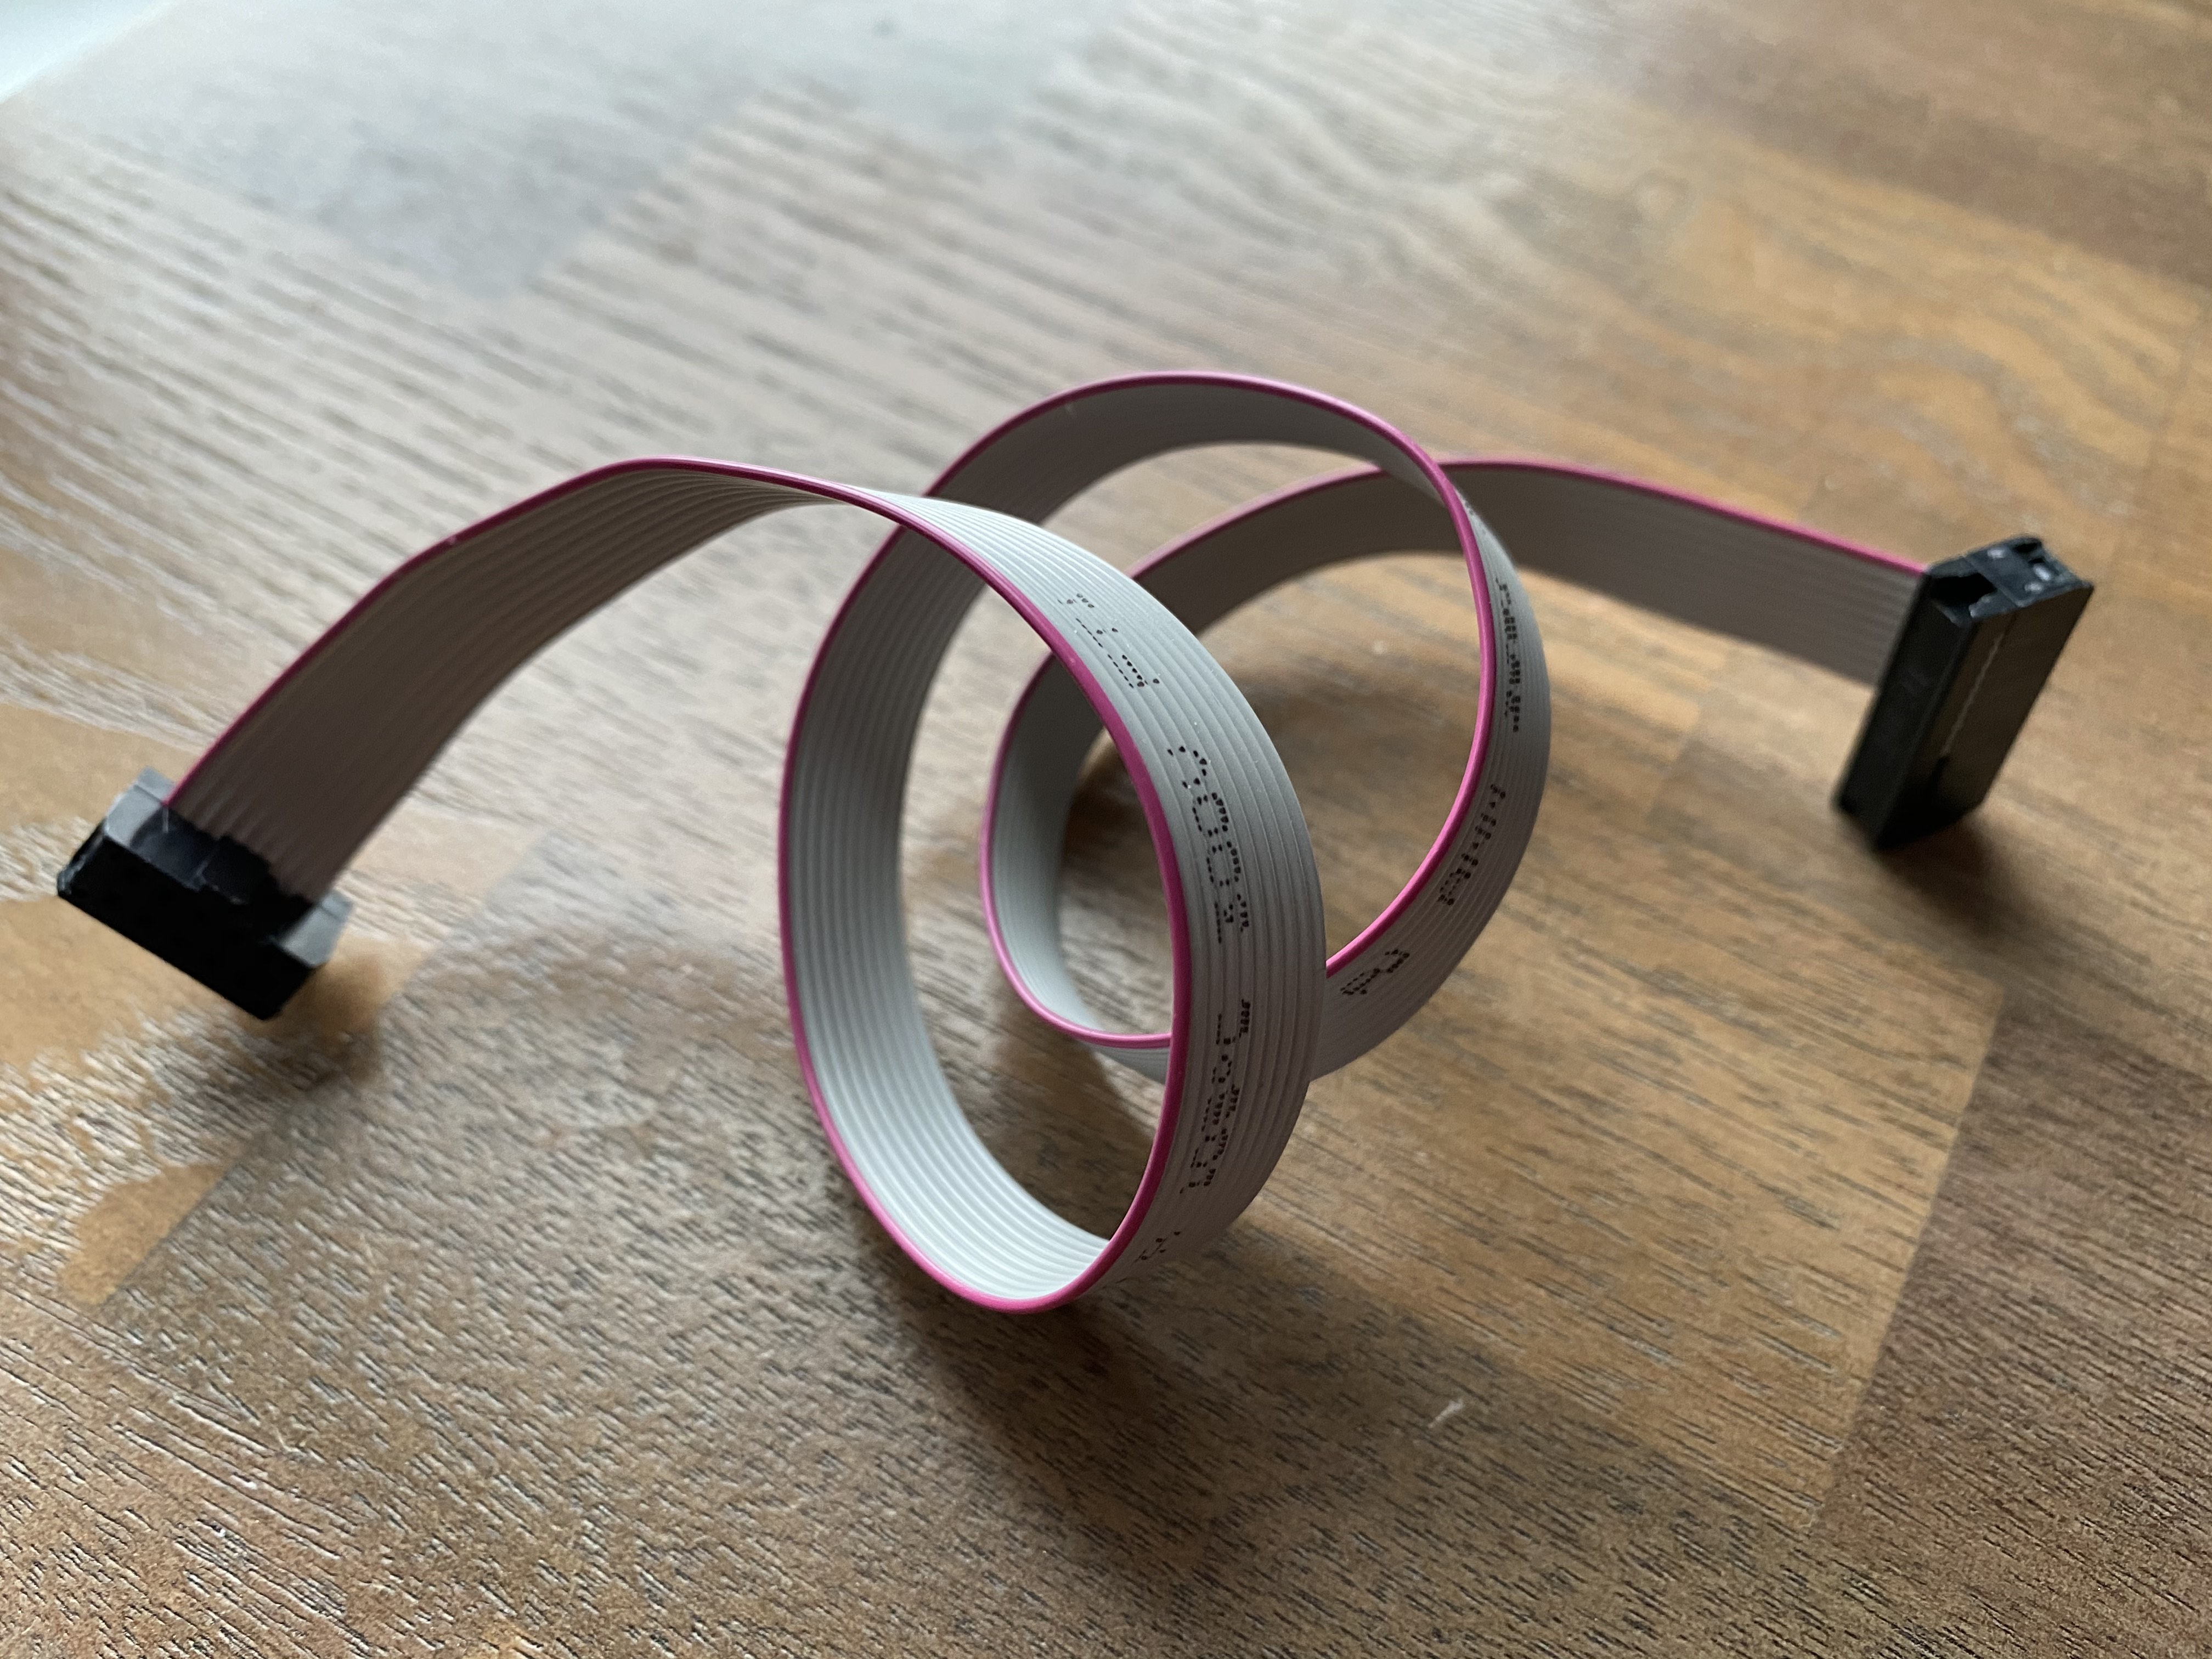
\includegraphics[width=1\linewidth]{../Images/Fig_Power_Cable_1}
	\caption{Eurorack Power Cable}
	\label{fig:power-cable}
\end{subfigure}%
\begin{subfigure}{.5\textwidth}
	\centering
	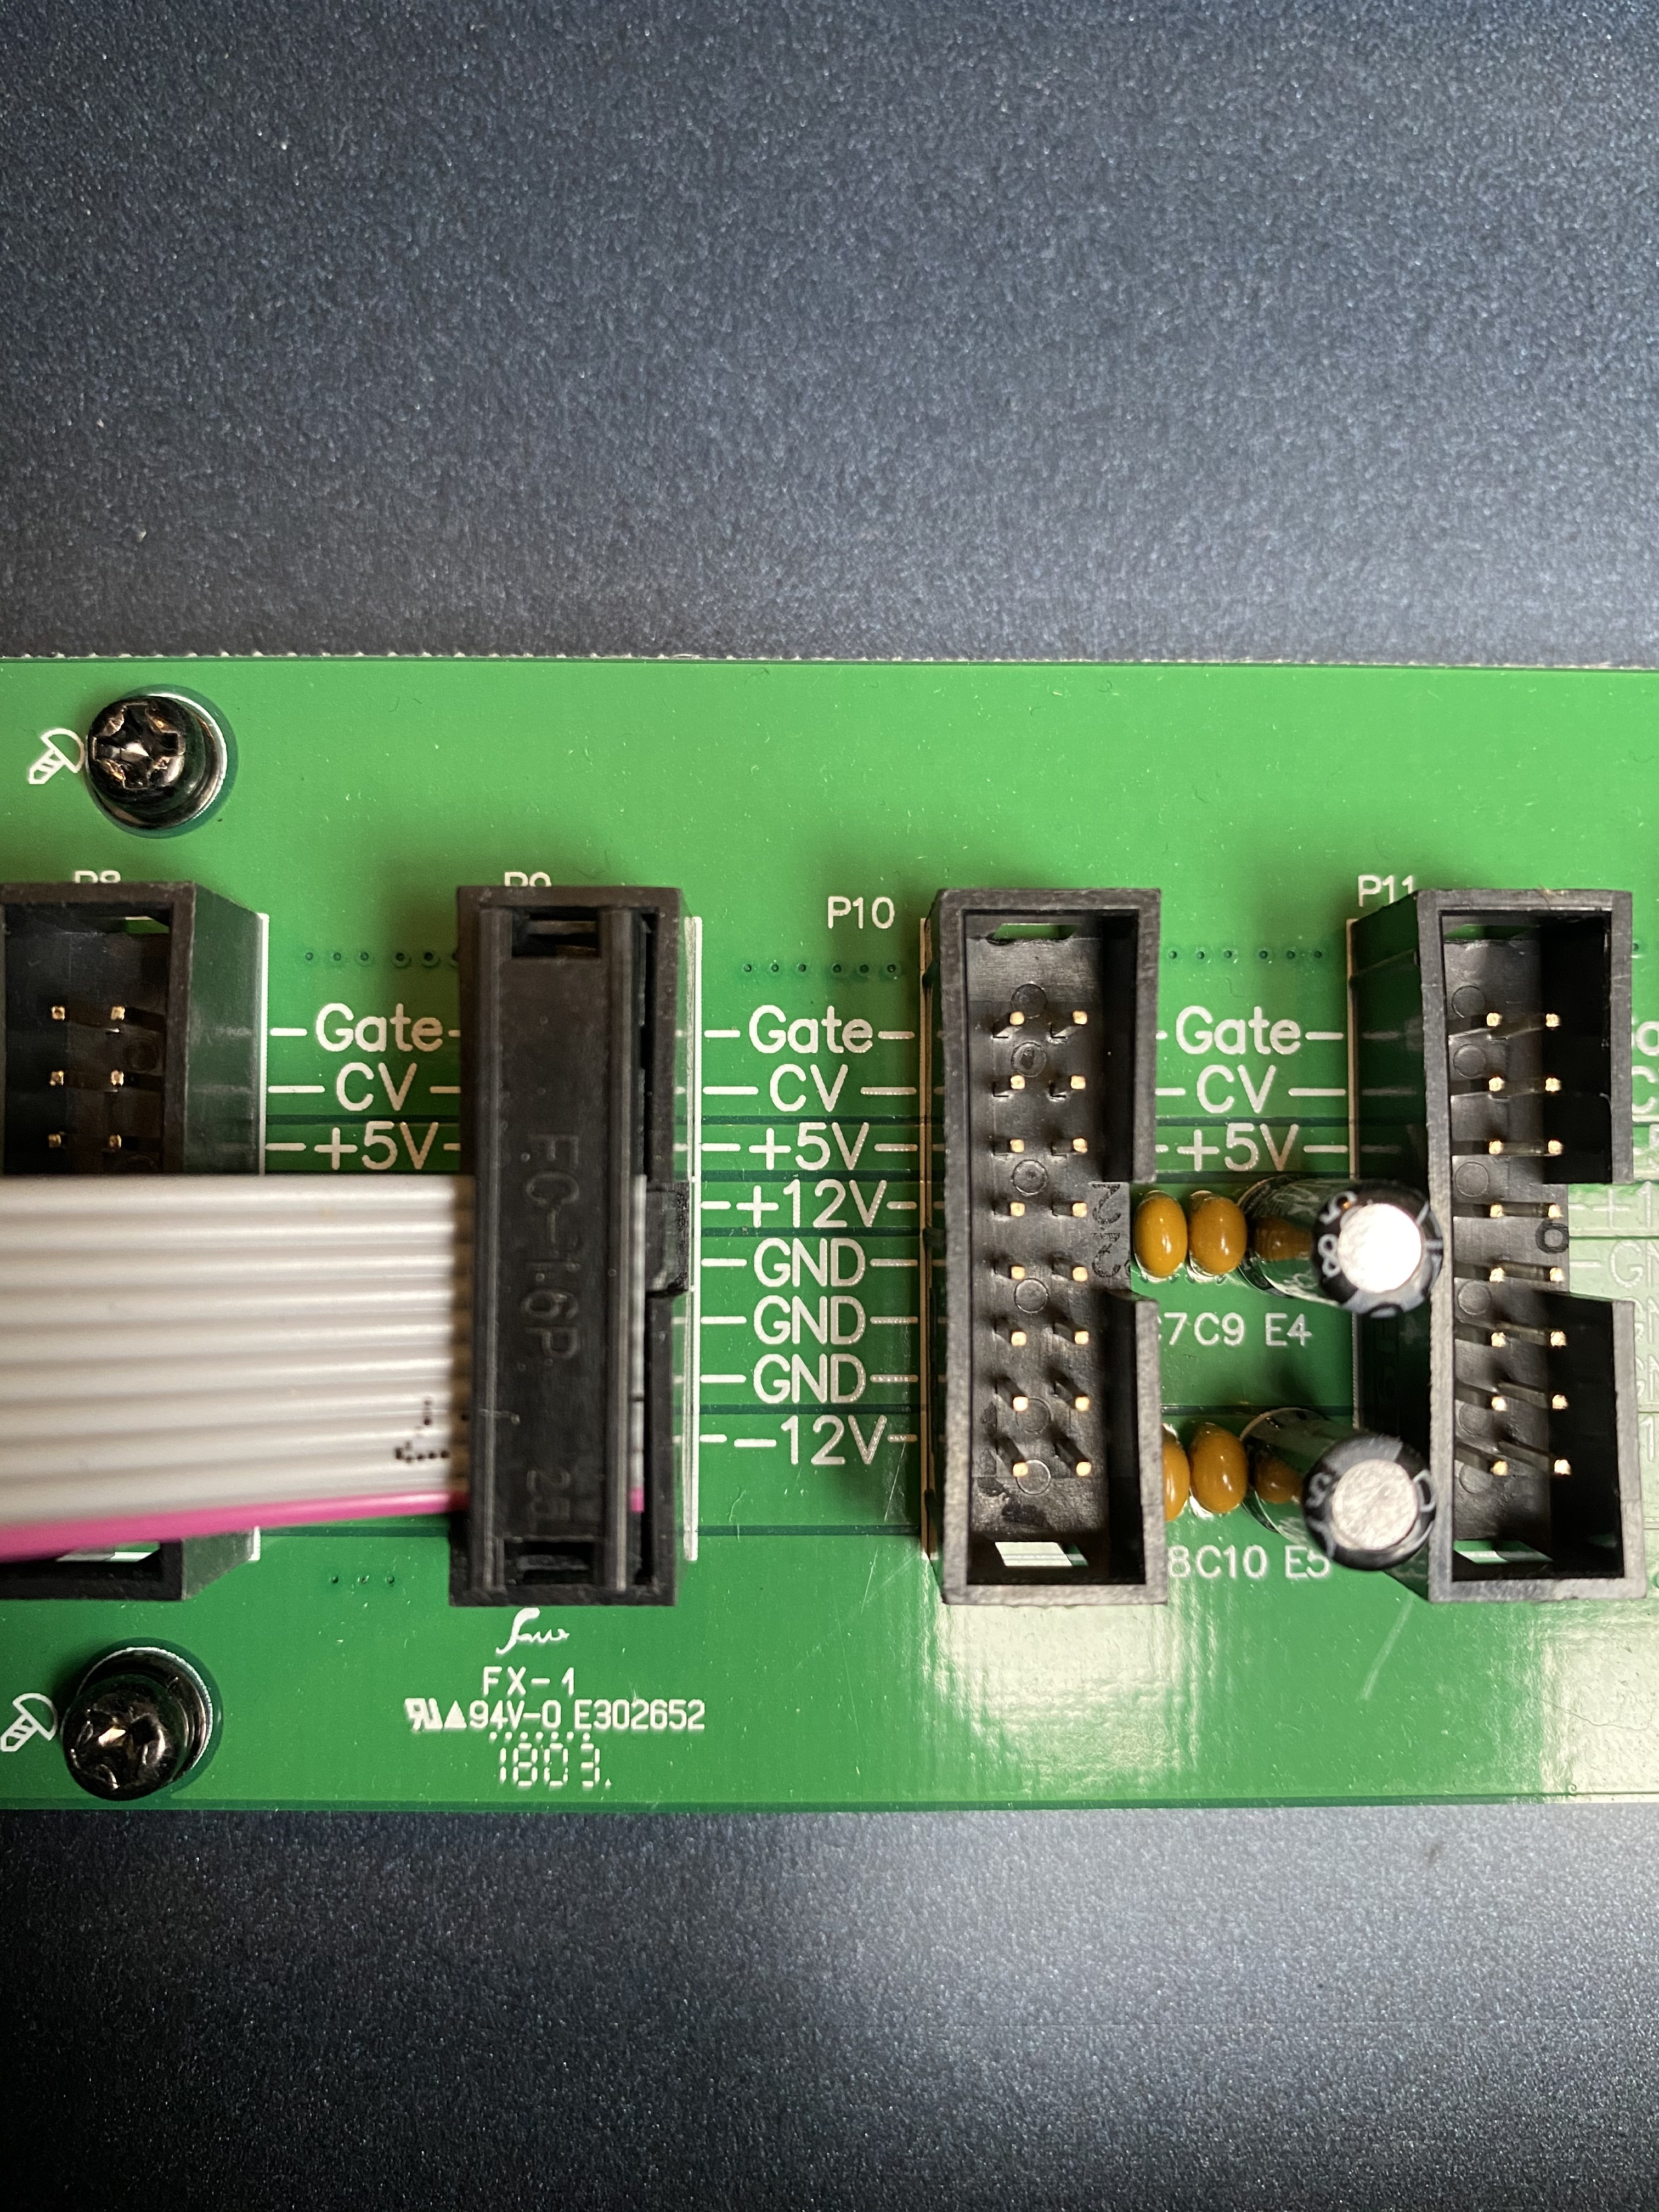
\includegraphics[width=0.8\linewidth]{../Images/Fig_Power_Bus}
	\caption{Eurorack power bus connector}
	\label{fig:power-bus}
\end{subfigure}
\caption{Eurorack power cable and power bus}
\end{figure}
\noindent When I began building my own modules I kept running out of power cables. These power cables bring the +/- 12V DC from your Eurorack power supply to the module. Most DIY retailers will include a power cable with their kits, but if you're starting from square one (i.e. getting your own PCBs manufactured) you will need to either buy or make some. These cables can be a bit pricey, so thankfully there is a very easy way to make them yourself.\\
\newline
\begin{note}
Our recommendation would be to purchase these items along with the components you will need for the power supply, which is the first module that we will be building.
\end{note}
\vspace{0.8cm}
\noindent \textbf{Below are the steps for building your own power cables}:
\begin{enumerate}
	\item Purchase an IDC crimping tool that can crimp the connectors on each end of the cable. I use \href{https://www.amazon.com/Eowpower-Crimp-Ribbon-Cable-Connectors/dp/B072MM8X7Y/ref=sr_1_2_sspa?dchild=1&keywords=IDC+crimp+tool&qid=1602446375&sr=8-2-spons&psc=1&spLa=ZW5jcnlwdGVkUXVhbGlmaWVyPUExMVpQUjRCMDNPRTE3JmVuY3J5cHRlZElkPUEwOTA3OTM2UEpBMU5OVERDVFJDJmVuY3J5cHRlZEFkSWQ9QTAwNzI1NzBWMVhWV1ZVRVBGTE0md2lkZ2V0TmFtZT1zcF9hdGYmYWN0aW9uPWNsaWNrUmVkaXJlY3QmZG9Ob3RMb2dDbGljaz10cnVl}{this one}, and despite some of the negative reviews, it works perfectly fine for our purposes.
	\item Purchase the connectors and raw cable (links below). \textbf{NOTE:} If you plan on moving forward to the first build, which is the Power Supply, then make sure to order these parts in addition to what is necessary for that build. No reason to pay shipping twice.
	\begin{itemize}
		\item \href{https://www.taydaelectronics.com/idc-socket-connector-2-54mm-2-5-pin.html}{10-Pin IDC Socket Connector} - It is typical for most Eurorack modules to utilize a 10 pin box header connector like the one shown in Figure~\ref{fig:10-pin-connector}. So, one end of our cable will plug into this socket.
		\begin{figure}[h]
			\centering
			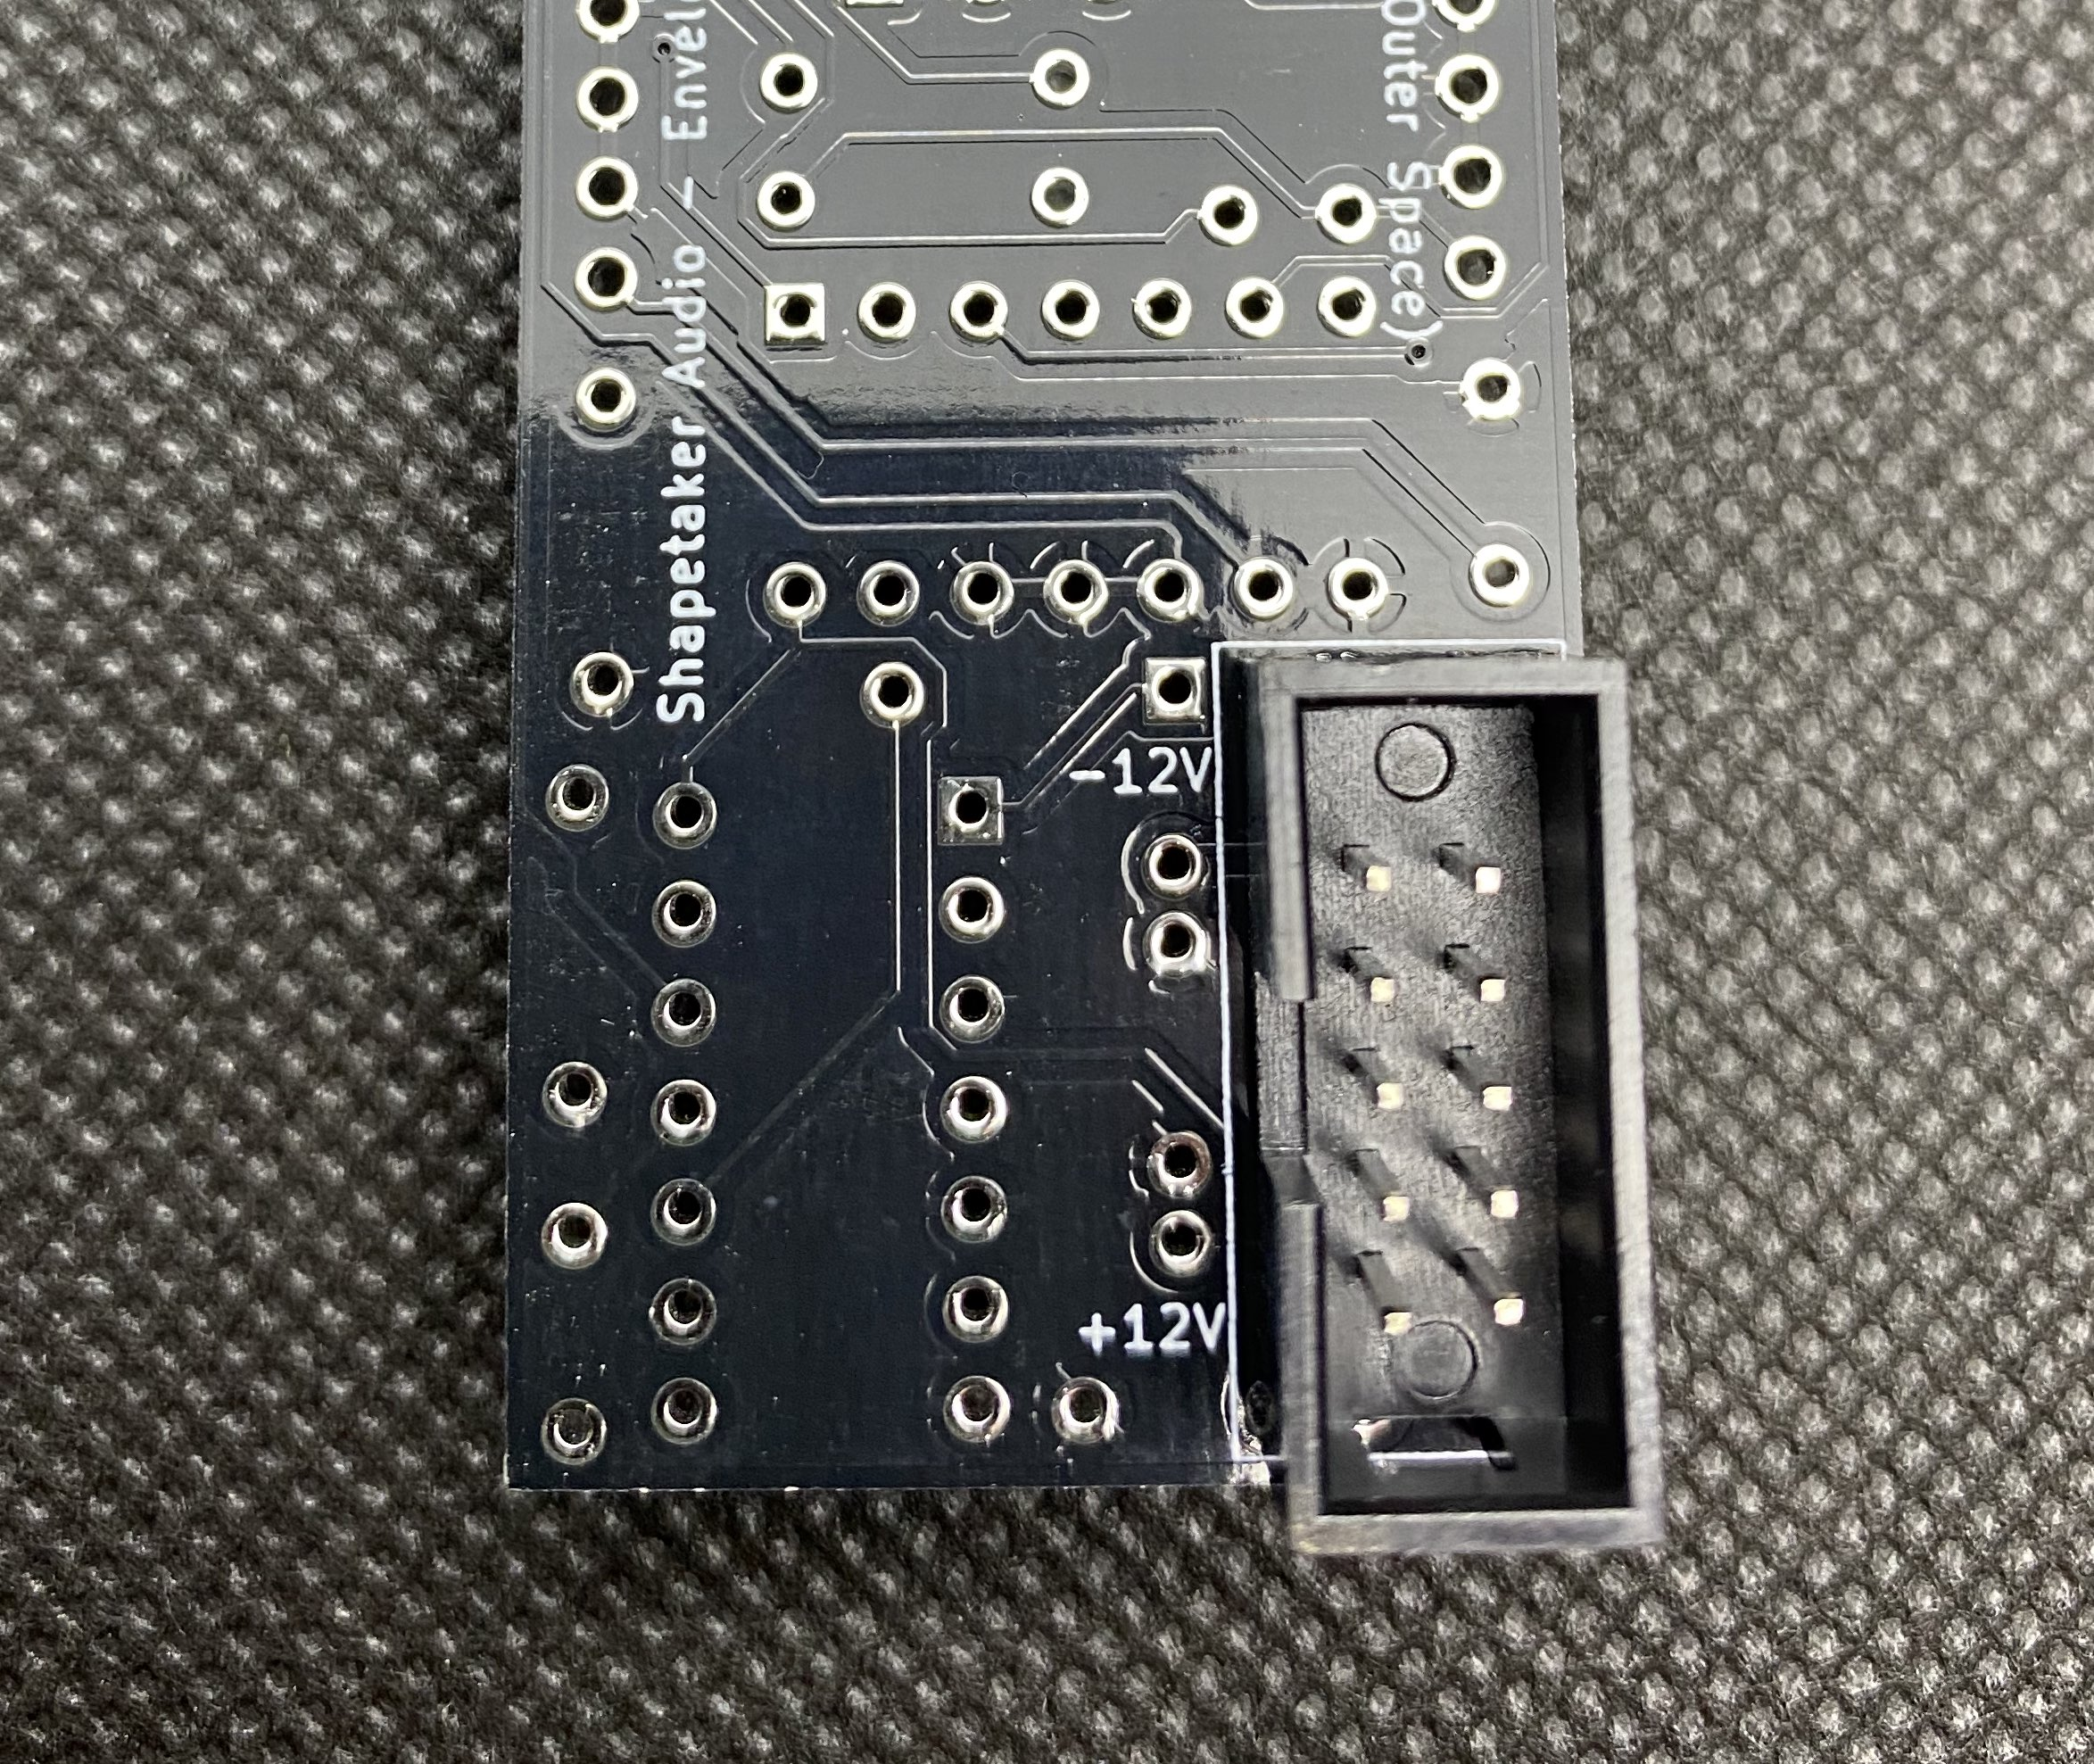
\includegraphics[width=.5\textwidth]{../Images/Fig_10_Pin_IDC}
			\caption{10 Pin IDC Box Header Connector}
			\label{fig:10-pin-connector}
		\end{figure}
		\item \href{https://www.taydaelectronics.com/idc-socket-connector-2-54mm-2-8-pin-single-contact..html}{16-Pin IDC Socket Connector} - Power buses for Eurorack are typically 16-pin because in addition to the +12V, -12V, and ground buses, they also carry +5V, CV, and Gate signals. You can see this type of connector in Figure~\ref{fig:power-bus} These are hardly ever used in practice, so I assume the convention just stuck.
		\item \href{https://www.taydaelectronics.com/awg-28-10-conductor-flat-ribbon-cable-1ft-30cm.html}{Raw 10 Conductor Cable} - This is 10 conductor flat ribbon cable that can be seen in both Figure~\ref{fig:power-cable} and ~\ref{fig:power-bus}. This cable is sold by the foot, and the standard sizes on Thonk are:\\
		\begin{itemize}
			\item Micro: 8cm (\textasciitilde1/4 ft)
			\item Short: 17cm (\textasciitilde0.5 ft)
			\item Long: 30cm (1ft)
			\item XL: 0.5m (\textasciitilde1.6 ft)
		\end{itemize}
	\vspace{0.3cm}
	But since you are making these, feel free to make them any size you like!
    \end{itemize}
\item Ensure that the notch on the 16 pin connector is facing away from you as shown in Figure ?.
\missingfigure[figwidth=10cm]{Pic ref - 1.1.1}
\item Align the red conductor of the ribbon cable with the rightmost conductor on connector and thread the cable through as shown in Figure ?.
\missingfigure[figwidth=10cm]{Pic ref - 1.1.2}
\item Ensure that the center of each conductor of the ribbon cable aligns with the terminal contact of the connector before crimping.
\missingfigure[figwidth=10cm]{Pic ref - 1.1.3}
\item Place the assembly between the crimping tool as shown in Figure ?.
\missingfigure[figwidth=10cm]{Pic ref - 1.1.4}
\item Press down firmly to force the terminal contacts to break the insulation of ribbon cable, therefore creating a solid connection.
\missingfigure[figwidth=10cm]{Pic ref - 1.1.5}
\item Remove the excess ribbon cable by cutting it with a side cutter, or knife.
\missingfigure[figwidth=10cm]{Pic ref - 1.1.6}
\item Repeat Steps 1-8 for the 10 pin connector.
\missingfigure[figwidth=10cm]{Pic ref - 1.1.7}
\item Test the continuity (connection resistance) by using a multimeter <TODO - complete this>
\missingfigure[figwidth=10cm]{Pic ref - 1.1.8}
\end{enumerate}
\subsubsection{Patch Cables}
You can never have enough patch cables. All sizes and all colors. The quality and price of these will vary quite a bit based on the manufacturer. If you search Amazon for "Eurorack patch cables" you will come up with tons of results. I recommend trying two different types/packs to get an idea of the quality and go from there. You can also try one of the retailers listed in the References section (\ref{mod-retailers}). Wish there were more I can say about these besides get yourself a bunch (these unfortunately are a bit more difficult to DIY and may not be worth the effort).

\subsection{Bench and Workspace}
Here are a few things I would recommend having for your workspace. They are by no means necessary, but again, very helpful:
\begin{itemize}
	\item\href{https://www.amazon.com/Absorber-Remover-Extractor-Prevention-Soldering/dp/B07VWDN29F/ref=sr_1_1_sspa?dchild=1&keywords=soldering+fan&qid=1602440986&sr=8-1-spons&psc=1&spLa=ZW5jcnlwdGVkUXVhbGlmaWVyPUExTjNOVzNVMUdTTThNJmVuY3J5cHRlZElkPUEwMzY1NTE1MlpBMjY4TUhKWDFCMiZlbmNyeXB0ZWRBZElkPUEwOTY0NTU1MVA3SFRYMDdPWVIzMyZ3aWRnZXROYW1lPXNwX2F0ZiZhY3Rpb249Y2xpY2tSZWRpcmVjdCZkb05vdExvZ0NsaWNrPXRydWU=}{Fume Extractor} - This is necessary if you are soldering in an enclosed space with poor ventilation! You will want to minimize the amount of noxious fumes you ingest while soldering. Keep in ming that the smoke that is coming from the tip of your iron is not lead, but it is still not good for your health.
	\item\href{https://www.amazon.com/Kaisi-Insulation-Silicone-Position-Soldering/dp/B07DGVRYL3/ref=sr_1_5?dchild=1&keywords=electronics+mat&qid=1602441242&sr=8-5}{Silicon Work Mat} - This mat can help keep all of your components and tools organized while you work. The non-ESD ones are fairly prone to static so be careful when handling integrated circuits if you purchase a mat like this. I personally have never had a problem with it, and I have been using it for about 6 months at this point.
	\item\href{https://www.amazon.com/Helping-Soldering-Workshop-Non-slip-Weighted/dp/B07MDKXNPC/ref=sr_1_3?crid=AB1YXXLOA4I1&dchild=1&keywords=third+hand+soldering+tool&qid=1602441328&sprefix=third+hand+%2Caps%2C143&sr=8-3}{Thrid Hand Soldering Tool} - This tool is a huge convenience and the benefit is very obvious! I do not use one because I am a glutton for punishment...
\end{itemize}

\subsection{Rack or Case}
I once was in a very popular modular synth shop on the west coast, and a salesperson told me that when it comes to cases I should "measure my ambition" before purchasing one. I felt like this wasn't fantastic advice considering every new comer wants the one that looks like a wall of knobs and blinking lights. Problem is, that one costs \$2,000... for just the case.\\
\newline
It can be daunting to find something that suites your needs and is affordable enough to get going. In the first part of our series, we will be building a power supply. In that case (no pun, for real), you have the ability to acquire something somewhat cheaper (as long as there is room to mount a small additional PCB (the power supply power bus <TODO -link)>.\\
\newline
One of the first products that comes to mind is the \href{http://tiptopaudio.com/products/}{Tip Top Audio Z-Rails \& Ears}. Check the links on the bottom right in the DIY section.\\
\newline
Or you can go for something a little more solid, such as the \href{https://www.perfectcircuit.com/make-noise-skiff-eurorack-case-104hp.html}{Make Noise Unpowered 104HP Skiff}. And if none of these seem slick enough to fit your style, than check out some excellent DIY Eurorack cases on YouTube. I've gone down a few rabbit holes...

\section{Assemble Your Own Modular Series}
This section houses links to all of the GitHub repos that exist in the AYOM series. Each module will have a "Main Board," which is the PCB where most of the functional circuit exists, and a "Control Board," (minus the power supply) which is where the knobs, switches, and input/output jacks will live, and a panel. Please make sure to download the accompanying assembly guide on each Main Board page (this will include instructions to assemble the entire module, not just the Main or Control board).
\subsection{Power Supply}
\begin{itemize}
	\item \href{https://github.com/joshpanzarella/AYOM-Power-Supply}{Power Supply Main Board GitHub}
	\item \href{https://github.com/joshpanzarella/AYOM-Power-Supply-Panel}{Power Supply Panel GitHub}
	\item \href{https://github.com/joshpanzarella/AYOM-Power-Supply-Bus}{Power Supply Bus Board GitHub}
\end{itemize}
\subsection{VCO}
\emph{coming soon...}
\subsection{VCA}
\begin{itemize}
\item \href{https://github.com/joshpanzarella/AYOM-VCA}{Voltage Controlled Amplifier Main Board GitHub}
\item \href{https://github.com/joshpanzarella/AYOM-VCA-Control-Board}{Voltage Controlled Amplifier Control Board GitHub}
\item \href{https://github.com/joshpanzarella/AYOM-VCA-Panel}{Voltage Controlled Amplifier Panel GitHub}
\end{itemize}
\subsection{EG (Envelope Generator)}
\emph{coming soon...}
\subsection{LFO}
\emph{coming soon...}
\subsection{VCF}
\emph{coming soon...}
\subsection{Utilities Module}
\emph{coming soon...}

\section{References}

\subsection{Electronics}
\subsubsection{Retailers}
\begin{itemize}
	\item \href{https://www.taydaelectronics.com}{Tayda Electronics} - Very affordable electronics retailer. Their stock seems to have an emphasis on DIY electronics. We will be using them a lot (I have no affiliation with Tayda, just believe they offer a great selection at a great price).
	\item \href{https://www.digikey.com}{DigiKey} - Big box electronics retailer. You can get anything here, if you can find exactly what you need.
	\item \href{https://www.mouser.com}{Mouser} - Same as Digikey for the most part.
	\item \href{https://www.sparkfun.com}{Sparkfun} - Awesome DIY/hobby electronics retailer. They often have excellent breakout boards that help you evaluate some extremely small and difficult to solder integrated circuit.
	\item \href{https://www.adafruit.com}{Adafruit} - Similar to SparkFun, sometimes one has something the other doesn't!
\end{itemize}
\subsubsection{Software}
\begin{itemize}
	\item \href{https://kicad-pcb.org}{KiCad} - Open source cross platform electronics design suite. This software was used to design all PCBs in this series.
	\item \href{http://www.falstad.com/circuit/}{Falstad Circuit Simulator Applet} - Excellent applet for observing the operation of basic circuits.
	\item \href{https://www.analog.com/en/design-center/design-tools-and-calculators/ltspice-simulator.html#}{LTSpice} - Powerful and free circuit simulation based on SPICE (Simulation Program with Integrated Circuit Emphasis). This is a bit more advanced, but with there are tons of tutorial videos available.
\end{itemize}

\subsection{Software}
\begin{itemize}
	\item \href{https://vcvrack.com}{VCV Rack} - A Eurorack simulator to mess around with before diving into hardware (or after... that works too!).
\end{itemize}

\subsection{Modular Things}

\subsubsection{Companies}
\begin{itemize}
	\item \href{https://mutable-instruments.net}{Mutable Instruments} - Some of the coolest modules ever created and open source! If you know modular, you know Mutable Instruments.
	\item \href{https://www.skullandcircuits.com}{Skull \& Circuits} - Excellent classic designs and DIY friendly.
	\item \href{https://northcoastsynthesis.com}{North Coast Synthesis} - Extensive technical knowledge in the blog section, great designs, and open source.
\end{itemize}

\subsubsection{DIY}
\begin{itemize}
	\item \href{URL}{Music From Outer Space}
	\item \href{URL}{Yu Synth}
\end{itemize}

\subsubsection{Forums}
\begin{itemize}
	\item \href{https://www.muffwiggler.com/forum/index.php}{Muff Wiggler} - A forum with an incredible wealth of knowledge from the smartest crew in the game.
\end{itemize}

\subsubsection{Retailers}{\label{mod-retailers}
\begin{itemize}
	\item \href{URL}{Perfect Circuit}
	\item \href{URL}{Thonk}
	\item \href{URL}{Modular Addict}
\end{itemize}

\subsubsection{Publications}
\begin{itemize}
	\item \href{URL}{Waveform Magazine}
\end{itemize}

\subsection{Books}
\begin{itemize}
	\item \href{https://www.amazon.com/Art-Electronics-Paul-Horowitz/dp/0521809266/ref=sr_1_2_sspa?crid=18V4A99G9B1KF&dchild=1&keywords=the+art+of+electronics&qid=1602447510&sprefix=the+art+of+elec%2Caps%2C141&sr=8-2-spons&psc=1&spLa=ZW5jcnlwdGVkUXVhbGlmaWVyPUEyVUlMNDQ0QVlQQU1BJmVuY3J5cHRlZElkPUEwNDEwMjc0MjdEM1M1SVNOUjNUWCZlbmNyeXB0ZWRBZElkPUEwNDY1MTgyMUJJU0JXUk1WUTcwSiZ3aWRnZXROYW1lPXNwX2F0ZiZhY3Rpb249Y2xpY2tSZWRpcmVjdCZkb05vdExvZ0NsaWNrPXRydWU=}{The Art of Electronics: Third Edition} - The electronics bible. Simply one of the best text in existence for the subject.
\end{itemize}
\end{document}
